\documentclass[tikz,border=6pt]{standalone}
\usepackage[T1]{fontenc}
\usepackage[utf8]{inputenc}
\usepackage{pgfplots}
\usepgfplotslibrary{groupplots}
\usetikzlibrary{calc}
\pgfplotsset{compat=1.18}
\begin{document}
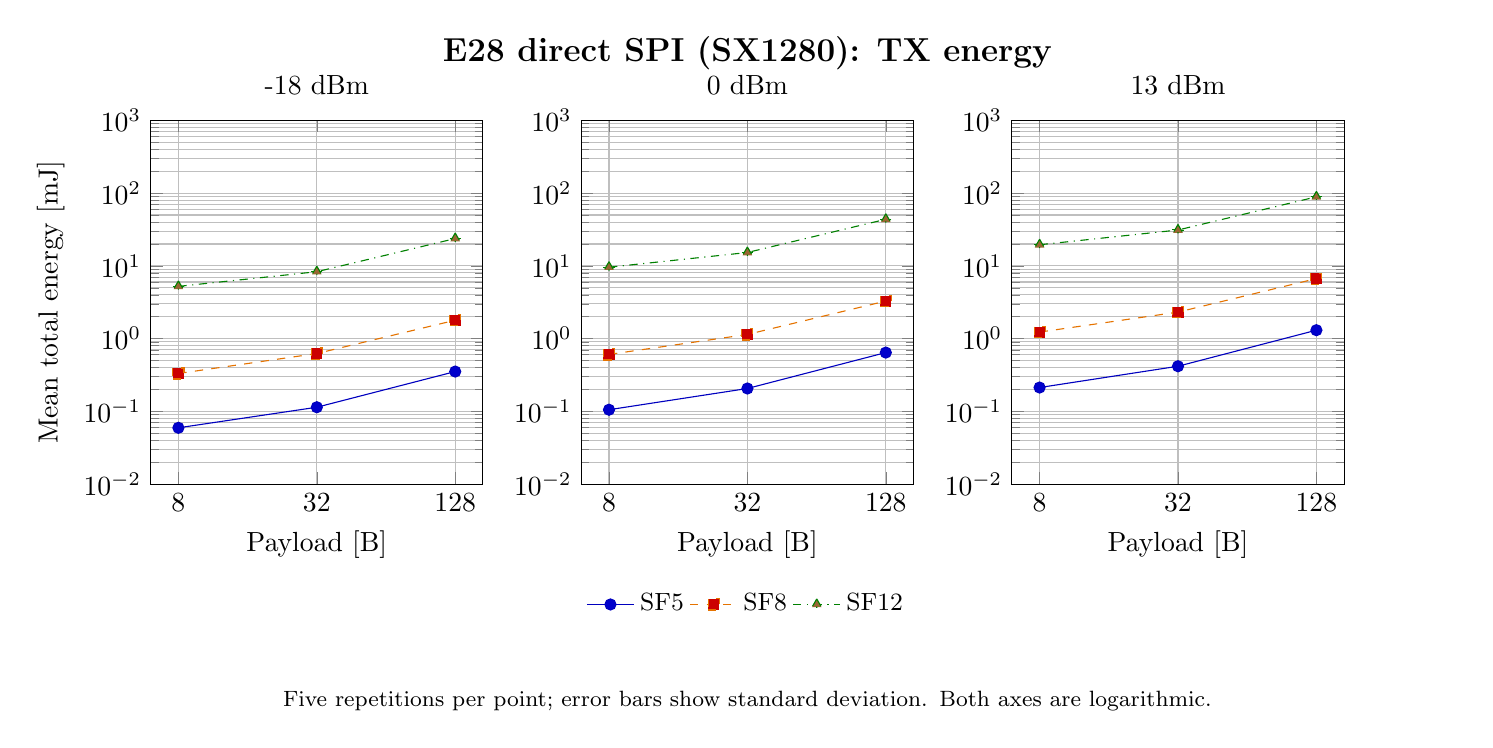
\begin{tikzpicture}
\begin{groupplot}[/pgf/number format/use comma, group style={group size=3 by 1, horizontal sep=1.25cm},
  width=5.8cm,height=6.2cm,xmode=log,log basis x=2,ymode=log,log basis y=10,ymin=0.01,ymax=1000,
  xtick={8,32,128},xticklabels={8,32,128},grid=both,xlabel={Payload [B]},
  legend style={draw=none,fill=none,font=\small,at={(0.5,-0.27)},anchor=north,legend columns=-1}]
% TX energy
\nextgroupplot[title={-18 dBm},ylabel={Mean total energy [mJ]}]
\addplot+[blue!75!black,solid,mark=*,error bars/.cd,y dir=both,y explicit] coordinates {(8,0.0593824206) +- (0,0.000474440838) (32,0.113872205) +- (0,0.0029782496) (128,0.352492541) +- (0,0.00202382211)};
\addplot+[orange!90!black,dashed,mark=square*,error bars/.cd,y dir=both,y explicit] coordinates {(8,0.331485186) +- (0,0.00120345065) (32,0.623684696) +- (0,0.00153897387) (128,1.78981299) +- (0,0.00540547299)};
\addplot+[green!50!black,dashdotted,mark=triangle*,error bars/.cd,y dir=both,y explicit] coordinates {(8,5.22589956) +- (0,0.0145312236) (32,8.31540161) +- (0,0.0240568441) (128,23.7679764) +- (0,0.0567085875)};
\nextgroupplot[title={0 dBm}]
\addplot+[blue!75!black,solid,mark=*,error bars/.cd,y dir=both,y explicit] coordinates {(8,0.10525544) +- (0,0.000775936673) (32,0.20613856) +- (0,0.00069275918) (128,0.642764931) +- (0,0.00134970895)};
\addlegendentry{SF5}
\addplot+[orange!90!black,dashed,mark=square*,error bars/.cd,y dir=both,y explicit] coordinates {(8,0.606057735) +- (0,0.00109651833) (32,1.14107117) +- (0,0.00149458415) (128,3.28286842) +- (0,0.0035804317)};
\addlegendentry{SF8}
\addplot+[green!50!black,dashdotted,mark=triangle*,error bars/.cd,y dir=both,y explicit] coordinates {(8,9.58487424) +- (0,0.017181447) (32,15.2785635) +- (0,0.0119496817) (128,43.7300239) +- (0,0.0546164601)};
\addlegendentry{SF12}
\nextgroupplot[title={13 dBm}]
\addplot+[blue!75!black,solid,mark=*,error bars/.cd,y dir=both,y explicit] coordinates {(8,0.21244352) +- (0,0.00107057463) (32,0.416920492) +- (0,0.00175434231) (128,1.30580825) +- (0,0.00139394468)};
\addplot+[orange!90!black,dashed,mark=square*,error bars/.cd,y dir=both,y explicit] coordinates {(8,1.22908945) +- (0,0.00317393486) (32,2.31463865) +- (0,0.00788799703) (128,6.68808069) +- (0,0.0215877545)};
\addplot+[green!50!black,dashdotted,mark=triangle*,error bars/.cd,y dir=both,y explicit] coordinates {(8,19.522688) +- (0,0.0579098323) (32,31.142606) +- (0,0.0983942111) (128,89.0247703) +- (0,0.274420996)};
\end{groupplot}
\node[font=\bfseries\large] at ($(group c2r1.north)+(0,0.85cm)$) {E28 direct SPI (SX1280): TX energy};
\node[font=\footnotesize,align=center,text width=18cm] at ($(group c2r1.south)+(0,-2.75cm)$) {Five repetitions per point; error bars show standard deviation. Both axes are logarithmic.};
\end{tikzpicture}
\end{document}
